\chapter{Evaluation}
In this chapter, we analyse the performance impact of the IOMMU, directly comparing it to the physical address approach. To compare both approaches fairly, we allocate and map the memory upfront. The focus lies on the IOMMU itself and how it performs. All performance tests use the Container IOMMU API instead of IOMMUFD as it currently remains the widely adopted VFIO variant.

\section{Setup}
We use two systems two benchmark the driver's performance.
Both systems run Ubuntu 23.10 with Linux kernel version 6.5.0-42 and are NUMA systems which 2 nodes each. We adhere to NUMA-locality.

\begin{table}[H]
  \centering
  \begin{tabular}{lllrll}
    \textbf{CPU}                          & \textbf{Memory}                         & \textbf{NVMe}                         & \textbf{Capacity}                       & \textbf{Count}   \\
    \toprule

    \multirow{2}{*}{Intel Xeon E5-2660v2} & \multirow{2}{*}{\qty{251}{\gibi\byte}}  & \multirow{2}{*}{Samsung Evo 970 Plus} & \multirow{2}{*}{\qty{1}{\tera\byte}}    &
    \multirow{2}{*}{1}                                                                                                                                                                   \\
                                          &                                         &                                       &                                         &                & \\ \hline

    \multirow{2}{*}{AMD EPYC 7713}        & \multirow{2}{*}{\qty{1007}{\gibi\byte}} & \multirow{2}{*}{Samsung PM9A3}        & \multirow{2}{*}{\qty{1.92}{\tera\byte}} &
    \multirow{2}{*}{8}                                                                                                                                                                   \\
                                          &                                         &                                       &                                         &                & \\
    \bottomrule
  \end{tabular}

  \caption{Specifications of systems used in performance testing}
  \label{tab:servers}
\end{table}

\begin{table}[H]
  \centering
  \begin{tabular}{llrrrr}
    \multirow{2}{*}{\textbf{CPU}} & \multirow{2}{*}{\textbf{Clock}} & \multirow{2}{*}{\textbf{Cores}} & \multirow{2}{*}{\textbf{Virtualization}} & \multirow{2}{*}{\textbf{Year}}
    \\
                                  &                                 &                                 &                                          &                                \\
    \toprule

    Intel Xeon E5-2660v2          & \qty{2.2}{\giga\Hz}             & 10                              & VT-d                                     & 2012                           \\
    AMD EPYC 7713                 & \qty{2.0}{\giga\Hz}             & 64                              & AMD-V                                    & 2021                           \\

    \bottomrule
  \end{tabular}

  \caption{CPUs of the systems}
  \label{tab:cpus}
\end{table}

\begin{table}[H]
  \centering
  \begin{tabular}{lrrll}
    \multirow{2}{*}{\textbf{NVMe}} & \textbf{Maximum}     & \textbf{Maximum}    & \multirow{2}{*}{\textbf{Turbowrite}} & \multirow{2}{*}{\textbf{Usage}} \\
                                   & \textbf{Queue Count} & \textbf{Queue Size} &                                      &                                 \\
    \toprule

    Samsung Evo 970 Plus           & 128                  & 16384               & Yes                                  & Consumer                        \\
    Samsung PM9A3                  & 128                  & 16384               & No                                   & Enterprise                      \\

    \bottomrule
  \end{tabular}

  \caption{NVMe(s) of the systems}
  \label{tab:nvmes}
\end{table}

Despite the NVMe specifications maximum capability of 65536 I/O queues, our SSDs support a more reasonable amount of 128 I/O queues, which seems to be a typical amount.
We use 1 thread per 1 I/O queue in our multithreaded tests. Turbowrite is a Samsung technology that drastically speeds up write latencies in the so-called "Turbowrite" buffer with the size of \qty{42}{\giga\byte} of the NVMe, as shown in \cite{vroom}. In order to use the Turbowrite NVMe to its maximum potential, most tests are conducted in said buffer to avoid the NVMe being the bottleneck instead of the IOMMU.
The NVMe SSDs are formatted to 512-byte blocksize. All writes are performed on an empty SSD to avoid any overhead through garbage collection on the NVMe. As the NVMe can optimize reads on an empty SSD, all reads will be performed on a full SSD. The tests mainly use random writes/reads, as the NVMe can drastically optimize sequential requests, which can lead to altered results.

We also disable Intel's pstate and AMD's frequency scaling driver options which can influence the results.

Additionally, all standard tests are run with the \texttt{iommu.strict=1} kernel parameter to ensure a flushed IOTLB.

\section{Impact of \qty{4}{\kibi\byte} pages}
\subsection{Throughput}
As Linux as well as our IOMMUs supports \qty{4}{\kibi\byte}, \qty{2}{\mebi\byte} and \qty{1}{\gibi\byte} page sizes we will first test and analyse how it affects the latencies and overall performance. Especially using \qty{4}{\kibi\byte} pages, a performance impact should be noticeable. As we use a typical unit size of \qty{4}{\kibi\byte} using \qty{4}{\kibi\byte} pages should result in TLB-thrashing, and every operation in a page walk.

When comparing the performance of vroom without the IOMMU against vroom with IOMMU using \qty{4}{\kibi\byte} and \qty{2}{\mebi\byte} pages on a 2MiB buffer, a performance difference of around 10\% can be observed. This stems from the aforementioned IOTLB-thrashing. Noticeable is that no performance impact can be seen when using a 4KiB buffer. This is because all pages can fit in the IOTLB.

\begin{figure}[H]
  \centering
  \subcaptionbox {1 \qty{4}{\kibi\byte} buffer per thread} {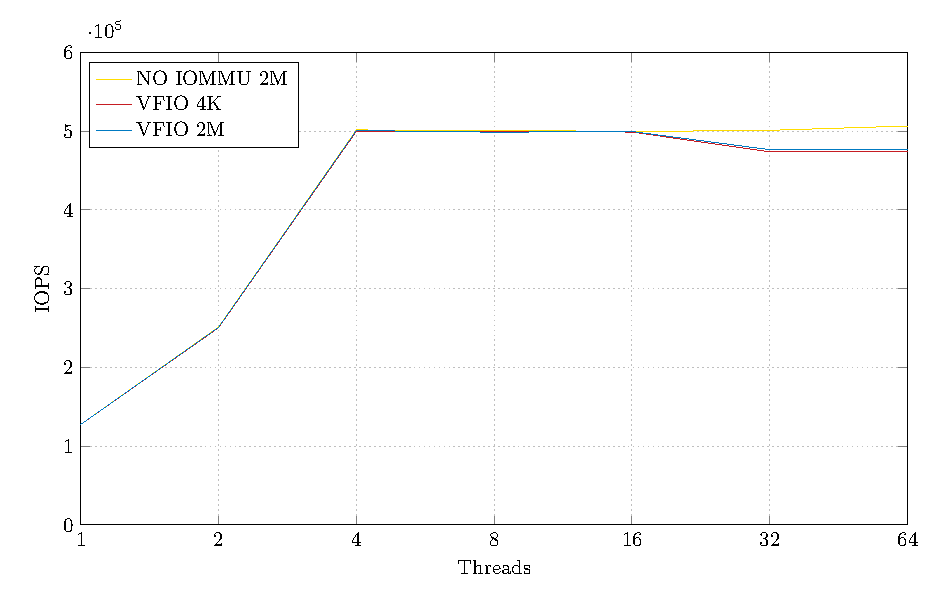
\includegraphics[width=0.75\textwidth]{figures/qd1tn_1page}}
  \subcaptionbox {1 \qty{2}{\mebi\byte} buffer per thread} {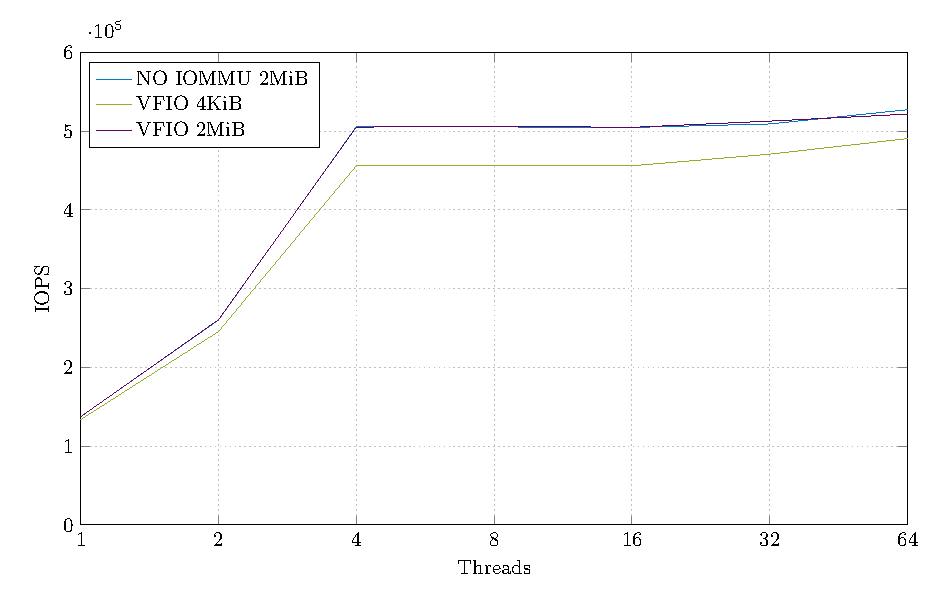
\includegraphics[width=0.75\textwidth]{figures/qd1tn_512page}}
  \caption{QD1 random write throughput over 20s with multithreading}
  \label{fig:qd1tn_4kib}
\end{figure}

\subsection{PCIe limitations}
When testing increasing queue depth, around a 10\% performance decrease can be seen using queue depth 4. When further increasing the queue depth, a decrease of this gap can be seen, with the throughput capping at around 890K IOPS.

The Intel System SSD is mounted on a PCIe 3.0 4x width bus with a maximum payload of 256 bytes. This PCI bus has a maximum throughput of 3.938 GB/s. Using the SSD to its full capability, i.e. using random writes with high queue depths in the Turbowrite buffer, can result in the bus being the bottleneck. With the highest throughput measured being 890K IOPS with one I/O operation containing 4096 bytes of data, we achieve 3.64 GB/s. Including the headers for each TLP and submission- and completion queue entries, we achieve 3.908 GB/s. This roughly equates the PCIe bus limits and leads us to conclude, that the missing overhead of using \qty{4}{\kibi\byte} pages stems from this bottleneck.

\begin{figure}[H]
  \centering
  \subcaptionbox {1 \qty{4}{\kibi\byte} buffer per thread} {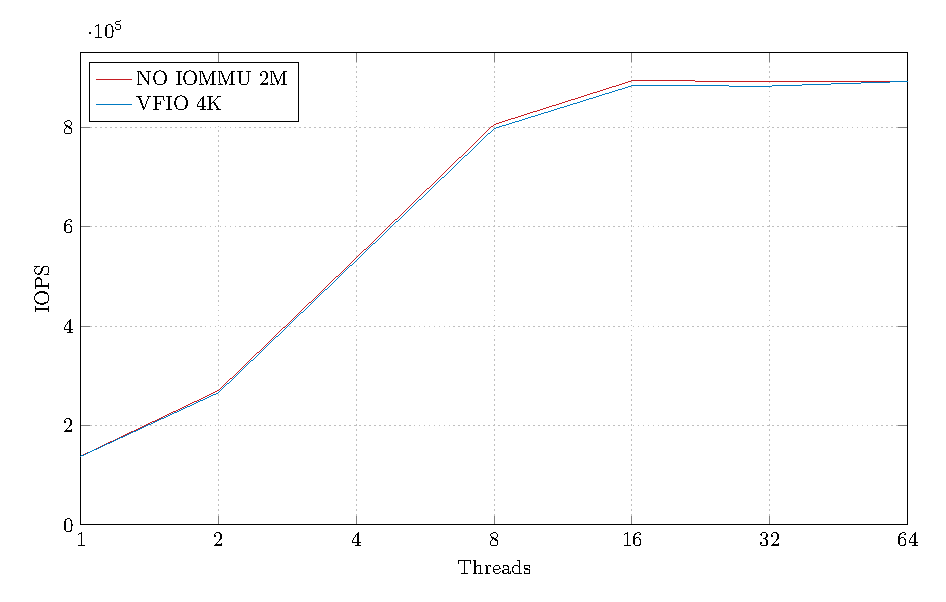
\includegraphics[width=0.48\textwidth]{figures/qdnt1_1page}}
  \subcaptionbox {1 \qty{2}{\mebi\byte} buffer per thread} {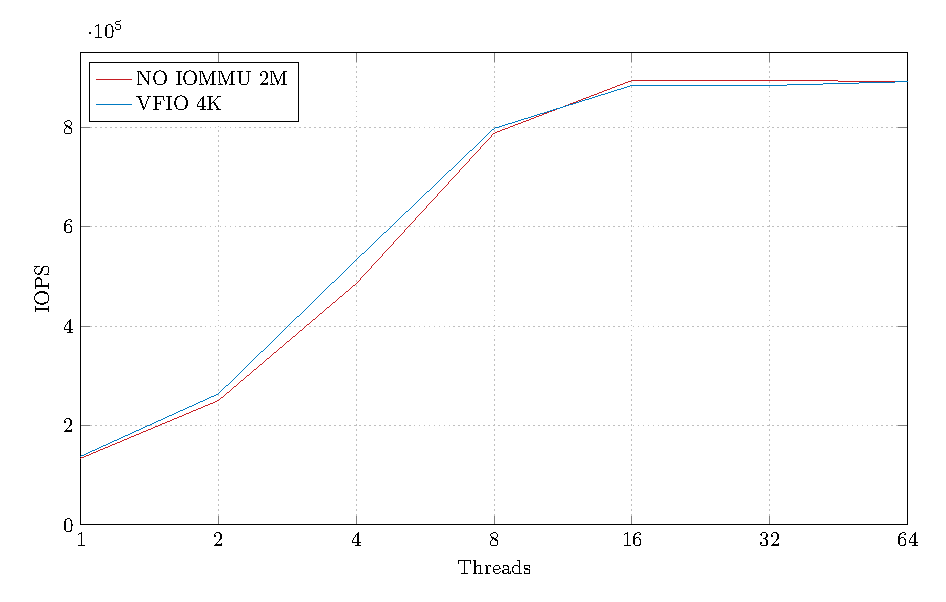
\includegraphics[width=0.48\textwidth]{figures/qdnt1_512page}}
  \caption{Singlethreaded random write throughput over 20s with increasing queue depth}
  \label{fig:qdnt1_4kib}
\end{figure}

\subsection{Determining IOTLB size}
As the size of the IOTLB is not stated in hardware and VT-d or AMD-V specifications, we use a latency test to analyze the behaviour of the IOMMU.
In order to isolate the effect of the IOMMU we track the latencies of the fastest operation the NVMe can perform. The fastest operation is using random writes with the smallest blocksize of \qty{512}{\byte}.

If we then write from a single block from each page to the NVMe, repeat it 65536 times on an increasing page count that are a power of two, we can figure out where a latency spike occurs. The page count right before the latency spike should equal the IOTLB entry count. We configure the queues, buffer and prp-list to each take up one page, resulting in 6 allocated pages before the actual workload, to not shift the latency spike over. This test is done using without the IOMMU with \qty{2}{\mebi\byte} pages and the IOMMU with \qty{4}{\kibi\byte}, \qty{2}{\mebi\byte} and \qty{1}{\gibi\byte} pages.

\paragraph{Results of Intel Xeon E5-2660v2}
In the resulting graph \autoref{fig:med-ps} we can observe a performance spike of around 250 nanoseconds for each write between 64 and 128 allocated pages. In the case of \qty{4}{\kibi\byte} pages, this is a memory size of only 512 KiB. Using this information, we can assume that the IOTLB has the same size for each pagesize, as well as it \textbf{being 64 entries of size}. This matches the page size Stefan Huber and Rolf Neugebauer found.

\begin{figure}[H]
  \centering
  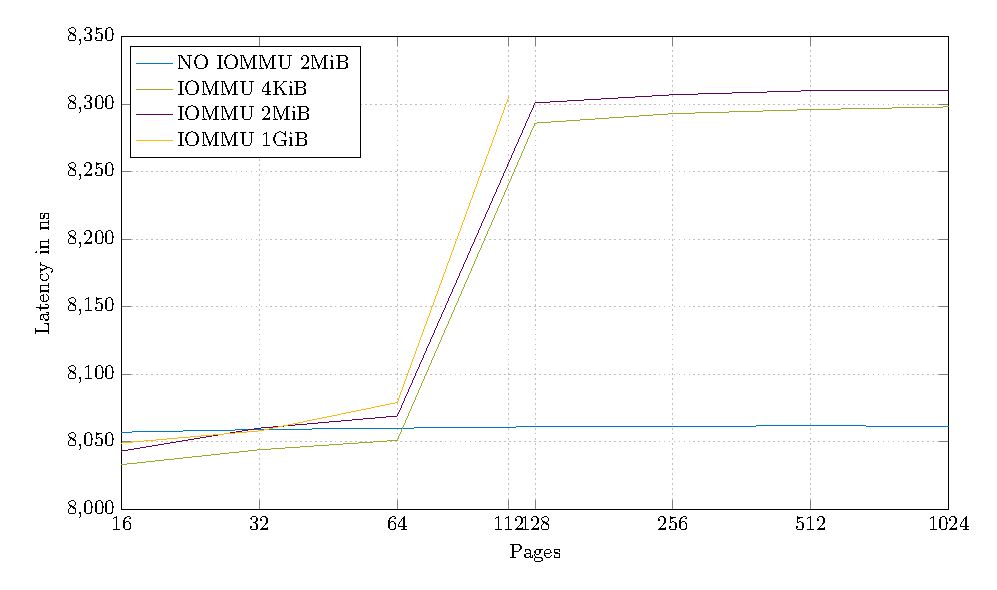
\includegraphics[width=\textwidth]{figures/psmeds}
  \caption{Latencies of random writes on an emptied SSD with increasing host memory pages on the Intel system}
  \label{fig:med-ps}
\end{figure}

\paragraph{Results of AMD EPYC 7713}
On the AMD IOMMU, we can see a performance spike that occurs at 64-128 pages for \qty{2}{\mebi\byte} and \qty{1}{\gibi\byte} page sizes and at 256-512 pages. We can therefore assume that the IOTLB size depends on the pagesize unlike on the Intel CPU. This leads us to suspect an \textbf{IOTLB size of 64 for \qty{2}{\mebi\byte} and \qty{1}{\gibi\byte} and 256 for \qty{4}{\kibi\byte} pages}. The performance itself only decreases by about \qty{60}{ns}, which is a five fold performance increase of page walks compared to the intel cpu system.

\begin{figure}[H]
  \centering
  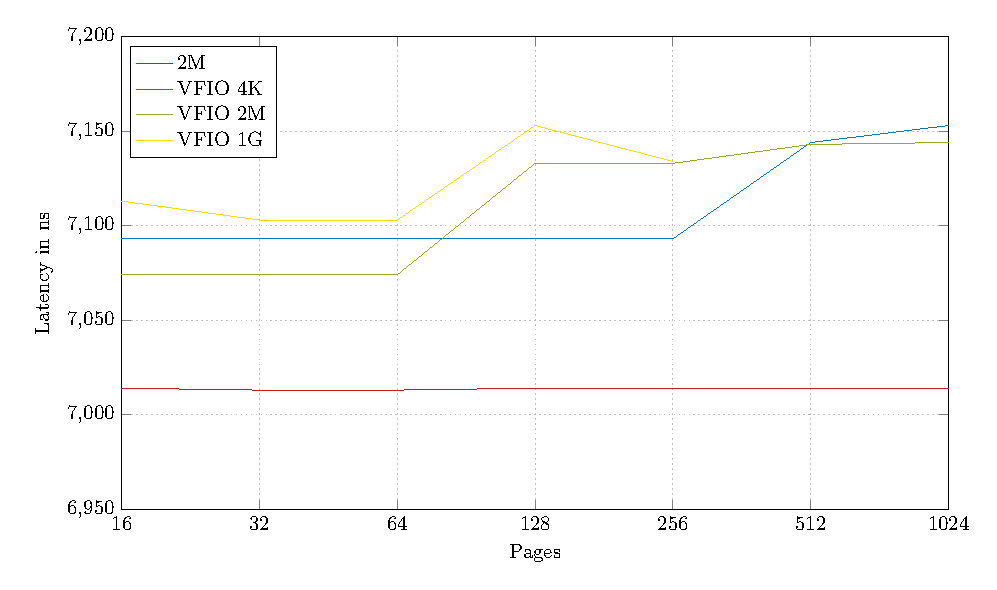
\includegraphics[width=\textwidth]{figures/psmedsepyc}
  \caption{Latencies of random writes on an emptied SSD with increasing host memory pages on the AMD system}
  \label{fig:med-psepyc}
\end{figure}

\section{Results}
For the following results, we will compare the latencies and throughput of vroom without the IOMMU and with the IOMMU, both utilizing \qty{2}{\mebi\byte} pages.

\subsection{Latencies}
\begin{figure}[H]
  \centering
  \subcaptionbox {Random read} {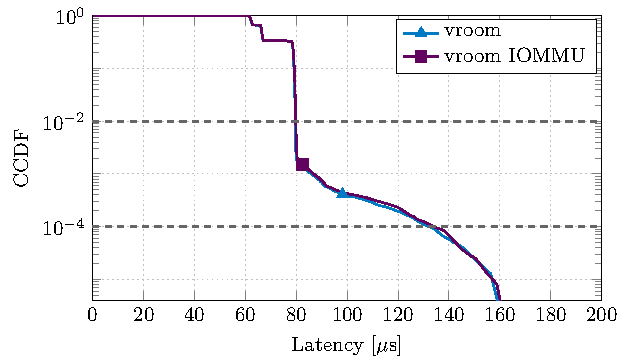
\includegraphics[width=.99\textwidth]{figures/lats_ccdf_2MiB_qd1t1_read} \label{fig:ccdf-read}}
  \subcaptionbox {Random write} {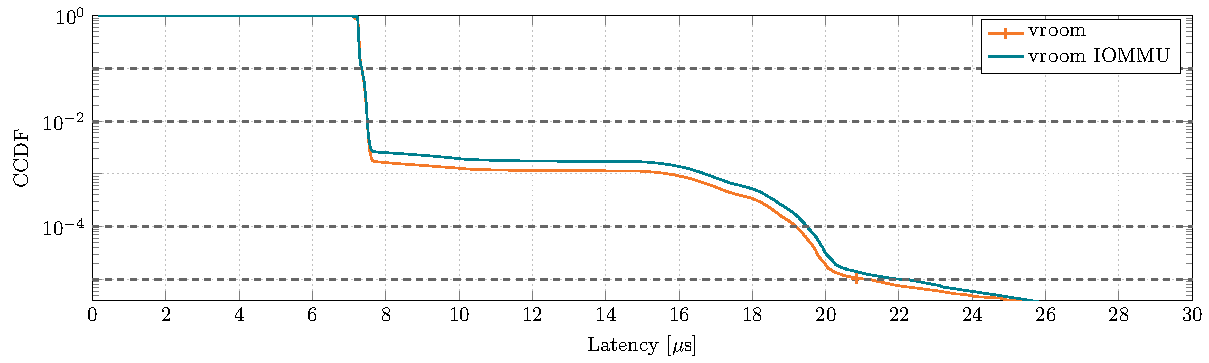
\includegraphics[width=.99\textwidth]{figures/lats_ccdf_2MiB_qd1t1} \label{fig:ccdf-write}}
  \caption{Tail latencies on Intel System}
  \label{fig:ccdf}
\end{figure}

\begin{figure}[H]
  \centering
  \subcaptionbox {Random read} {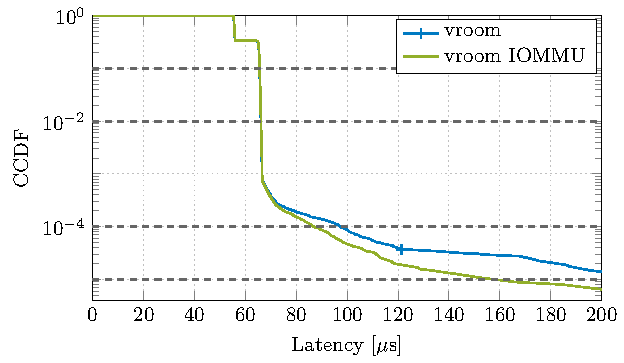
\includegraphics[width=.99\textwidth]{figures/lats_ccdf_2MiB_qd1t1_read_epyc} \label{fig:ccdf-read-epyc}}
  \subcaptionbox {Random write} {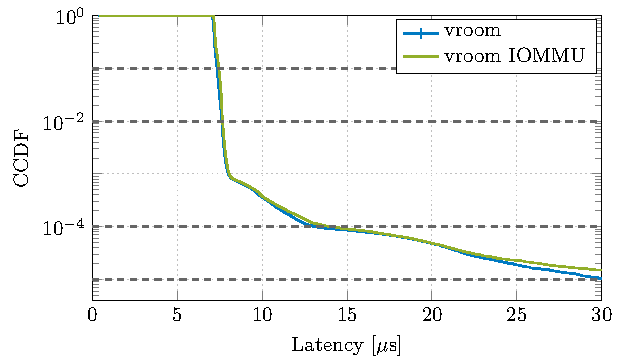
\includegraphics[width=.99\textwidth]{figures/lats_ccdf_2MiB_qd1t1_epyc} \label{fig:ccdf-write-epyc}}
  \caption{Tail latencies on AMD System}
  \label{fig:ccdf-epyc}
\end{figure}

\subsection{Throughput}
All throughput tests are done with a \qty{1}{\gibi\byte} buffer in memory. For \qty{2}{\mebi\byte} pages this equates to 512 pages being accessed.

% \begin{figure}[H]
%   \centering
%   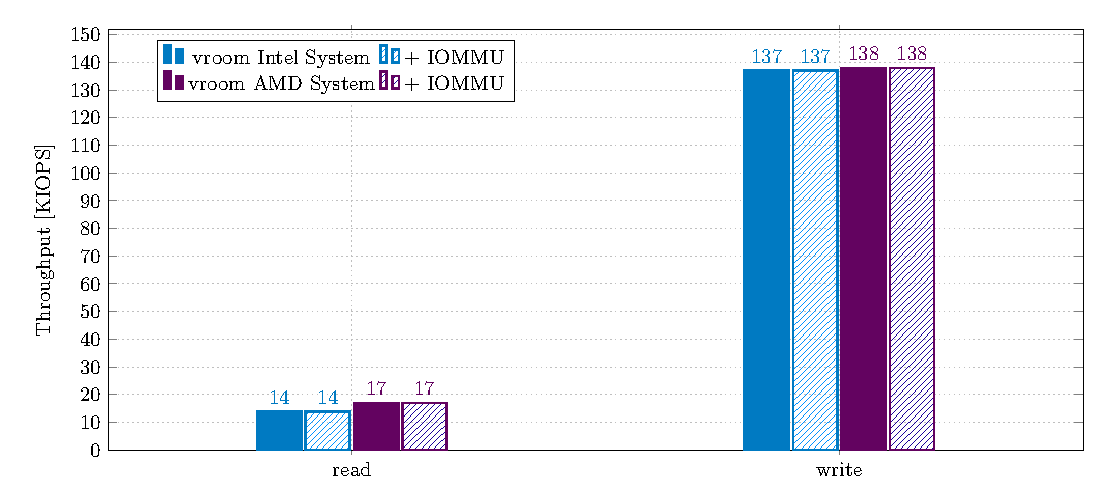
\includegraphics[width=.8\textwidth]{figures/throughput_bar_qd1t1}
%   \caption{Throughput over 60s with queue depth 1 and 1 thread}
%   \label{fig:throughput}
% \end{figure}

% \begin{figure}[H]
%   \centering
%   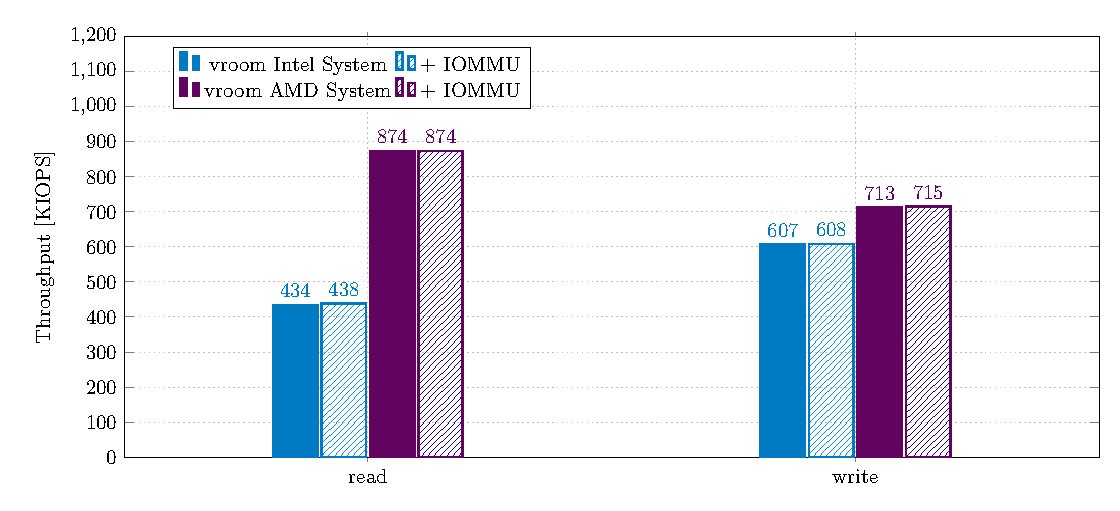
\includegraphics[width=.8\textwidth]{figures/throughput_bar_qd32t4}
%   \caption{Throughput over 60s with queue depth 32 and 4 threads}
%   \label{fig:throughputepyc}
% \end{figure}

\begin{figure}[H]
  \centering
  \subcaptionbox {Queue depth 1 and 1 thread} {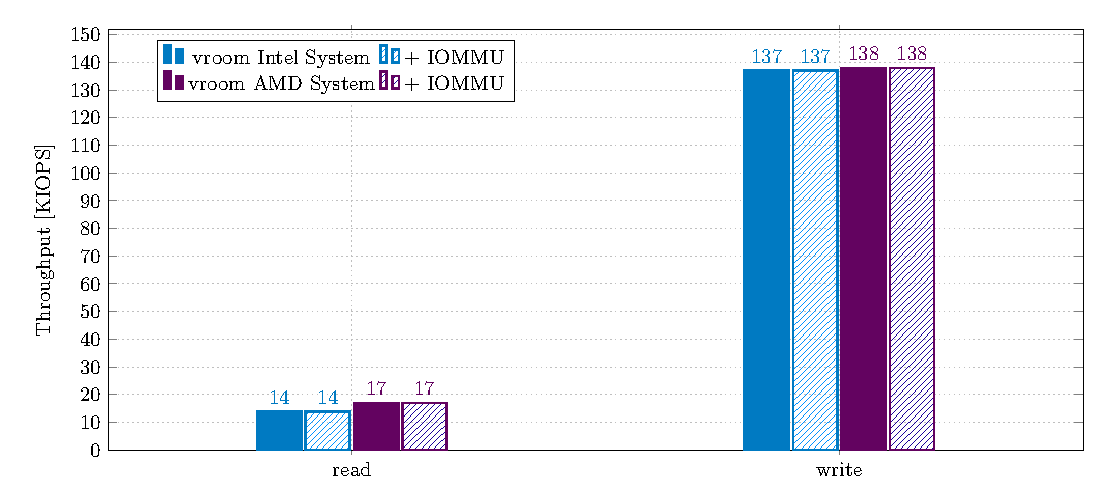
\includegraphics[width=.9\textwidth]{figures/throughput_bar_qd1t1} \label{fig:throughput-qd1t1}}
  \subcaptionbox {Queue depth 32 and 4 threads} {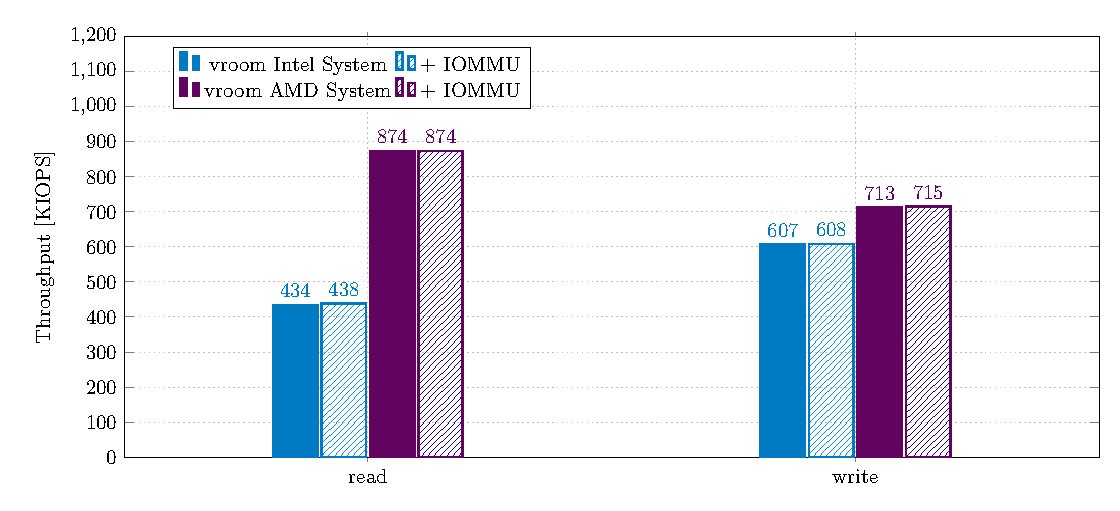
\includegraphics[width=.9\textwidth]{figures/throughput_bar_qd32t4} \label{fig:throughput-qd32t4}}
  \caption{Throughput over 60s}
  \label{fig:throughput-bar}
\end{figure}


We also take a look at throughput performance with larger queue depths. The queue depth describes how many outstanding requests are put onto a submission queue.

% \begin{figure}[H]
%   \centering
%   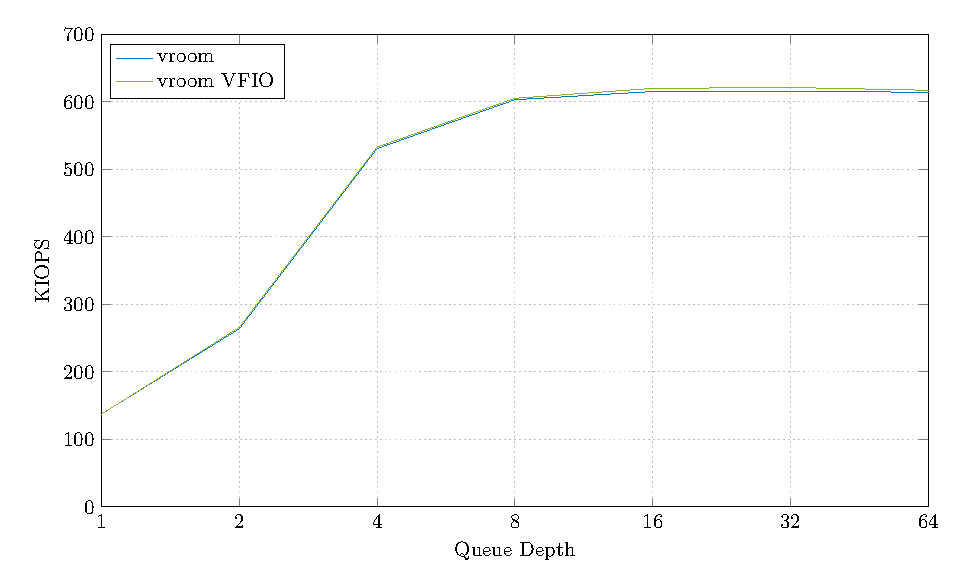
\includegraphics[width=.8\textwidth]{figures/qdnt1_2MiB}
%   \caption{Throughput with increasing Queue Depth on the Intel system}
%   \label{fig:qdnt1}
% \end{figure}

% \begin{figure}[H]
%   \centering
%   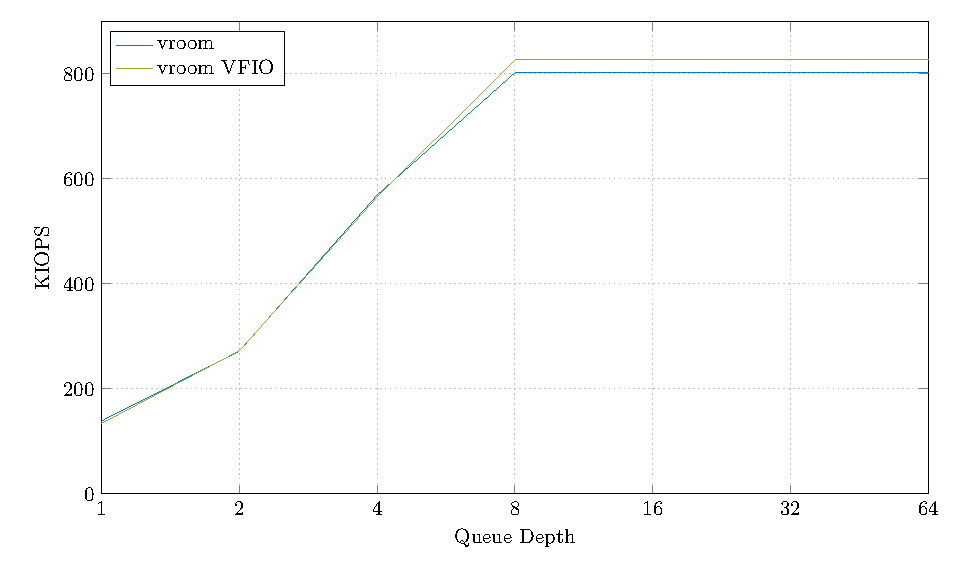
\includegraphics[width=.8\textwidth]{figures/qdnt1_2MiB_epyc}
%   \caption{Throughput with increasing Queue Depth on the AMD system}
%   \label{fig:qdnt1epyc}
% \end{figure}

\begin{figure}[H]
  \centering
  \subcaptionbox {Intel System} {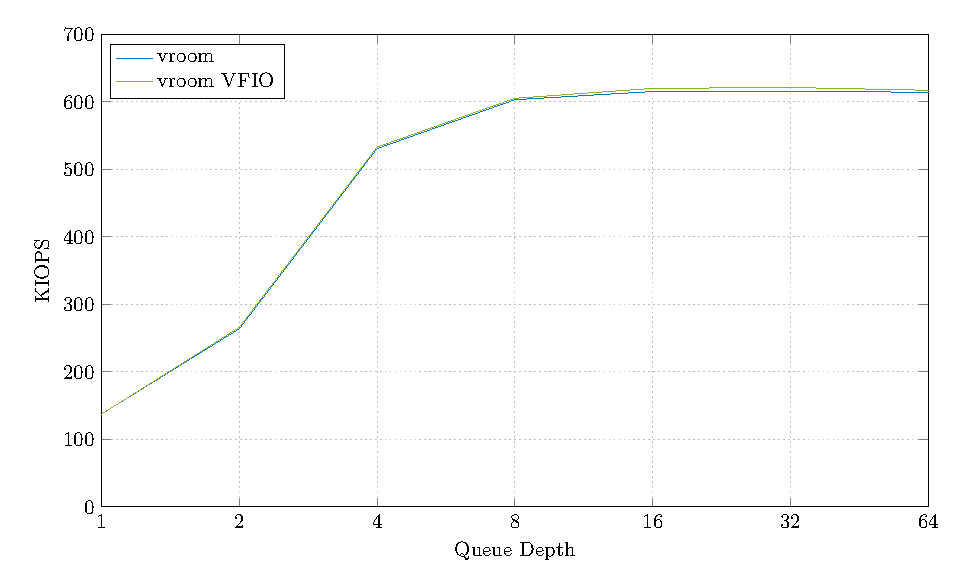
\includegraphics[width=.8\textwidth]{figures/qdnt1_2MiB} \label{fig:qdnt1-2MiB-intel}}
  \subcaptionbox {AMD System} {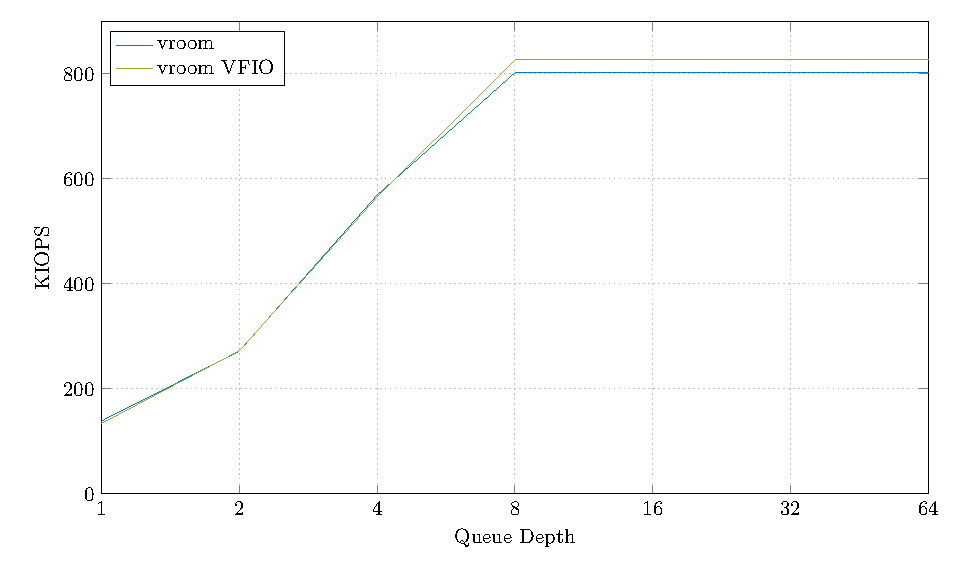
\includegraphics[width=.8\textwidth]{figures/qdnt1_2MiB_epyc} \label{fig:qdnt1-2MiB-epyc}}
  \caption{Throughput over 60s of random writes with increasing Queue Depth}
  \label{fig:qdnt1-2MiB}
\end{figure}

All tests with multiple SSDs are run on the system with the AMD CPU.

\begin{figure}[H]
  \centering
  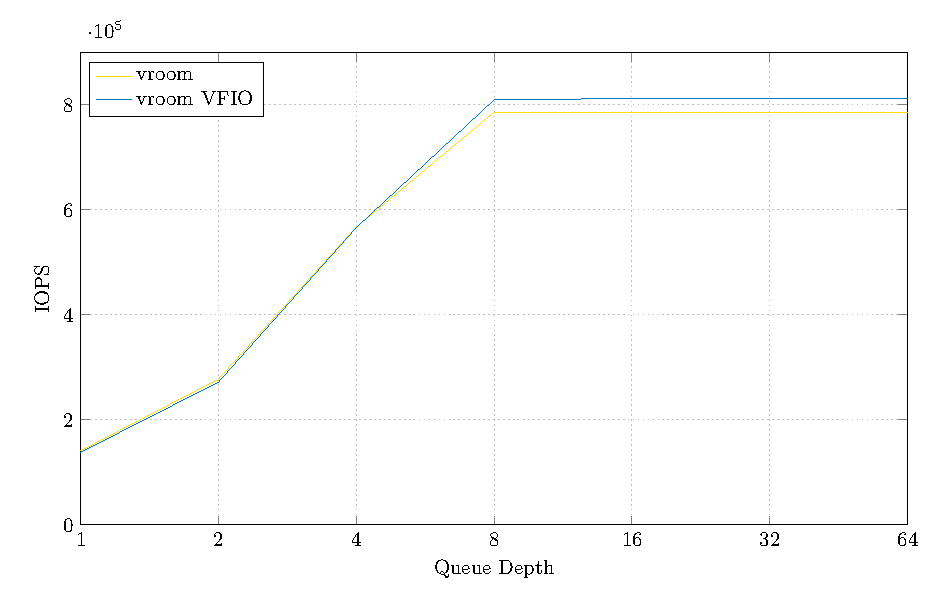
\includegraphics[width=\textwidth]{figures/qdnt1_2MiB_8nvmes}
  \caption{Throughput on 8 NVMe SSDs with 1 thread each}
  \label{fig:8nvmes}
\end{figure}

\section{IOMMU modes}
There are a couple of kernel parameters that can be set at boot-time to influence the behaviour of the IOMMU. The availability is influenced by the iommu manufacturer, e.g. theres \texttt{amd\_iommu} and \texttt{intel\_iommu}, as well as the CPU architecture. Many of these manufacturer dependent options are either very specific, or shared behaviour is ported to the general iommu parameter, e.g. \texttt{amd\_iommu=fullflush} and \texttt{intel\_iommu=strict}. We will be mainly looking at the general options \texttt{iommu}.

\paragraph{Strict}
To enable strict IOMMU mode, \texttt{iommu.strict=1} has to be set. Using strict mode, unmapping operation cause a complete IOTLB invalidation. Using relaxed mode, unmapping operations can be deferred and batched. This increases performance as an invalidation completely clears the IOTLB buffer, but reduces device isolation.

\paragraph{Passthrough}
Passthrough mode can be enabled using \texttt{iommu.passthrough=1}. Using passthrough DMA operations bypass the translation of the IOMMU, and instead directly access physical memory.